% chktex-file 13
\documentclass{beamer}
\usepackage[utf8]{inputenc}
\usepackage{datetime2}
\usepackage{multicol}
\usepackage{amssymb}
\usepackage{tikz}
\usetikzlibrary{shadows,arrows,fit,matrix,backgrounds}
\usepackage{calc}
\usepackage{booktabs}
\usepackage{makecell}
\usepackage[font=scriptsize]{caption}
\usepackage{csquotes}
\usepackage{xcolor}
\usepackage[ngerman]{babel}
\usetheme{metropolis}
\usepackage[
style=alphabetic,
citestyle=alphabetic,
sorting=nyt]{biblatex}
\addbibresource{literatur.bib}
\setbeamertemplate{frametitle continuation}{\insertcontinuationcount}
% % Definition Progressbar
\makeatletter
\newlength{\custom@progressinheadfoot}
\setbeamertemplate{progress bar in head/foot}{
	\nointerlineskip%
	\setlength{\custom@progressinheadfoot}{%
		\paperwidth * \ratio{\insertframenumber pt}{\inserttotalframenumber pt}%
	}%
	\begin{beamercolorbox}[wd=\paperwidth]{progress bar in head/foot}
		\begin{tikzpicture}
		\draw[bg, fill=bg] (0,0) rectangle (\paperwidth, 0.4em);
		\draw[fg, fill=fg] (0,0) rectangle (\custom@progressinheadfoot, 0.4em);
		\end{tikzpicture}%
	\end{beamercolorbox}
}
\addtobeamertemplate{footline}{}{%
	\usebeamertemplate*{progress bar in head/foot}%
}
\newcolumntype{C}[1]{>{\centering\let\newline\\\arraybackslash\hspace{0pt}}m{#1}}
\tikzset{
    block/.style    = { rectangle, draw=blue, thick, 
	fill=blue!20, text width=4em,
	rounded corners,execute at begin node=\setlength{\baselineskip}{8pt} },
	line/.style     = {draw, thick, ->},
	block2/.style = {block, text width= 6em},
	block3/.style = {block, text width=0.7\textwidth, drop shadow, minimum height=1.5em},
	block4/.style = {block, minimum height=2.2em, drop shadow},
	block5/.style = {block, drop shadow, text centered},
	line2/.style = {line, <->},
}
{
	\tikzset{terminal/.append style={text height=1.5ex,text depth=.25ex}}
	\tikzset{nonterminal/.append style={text height=1.5ex,text depth=.25ex}}
}
\nocite{factor}
\title{12 Factor App}
\subtitle{Eine Methode zur Entwicklung einer Software-as-a-Service (SaaS) Applikation}
\author{Sidney Kuyateh \& Steffen Walter}
\institute{Duale Hochschule Baden-Württemberg}
\date{\today}
\setbeamercolor{progress bar in head/foot}{fg=orange, bg=lightgray}
\begin{document}
	\maketitle
	\AtBeginSection{
		\begin{frame}{Überblick}
			\scriptsize
			\setlength{\baselineskip}{7pt}
			\vspace{0.3cm}
			\tableofcontents[sectionstyle=show, subsectionstyle=show/shaded,currentsection]
		\end{frame}
}
	\begin{frame}{Überblick}
		\scriptsize
		\setlength{\baselineskip}{7pt}
		\vspace{0.3cm}
		\tableofcontents
		\vfill
	\end{frame}
			%%%% Steffen %%%%
		\section{Einführung}
			\metroset{block=fill}
			\subsection{Einführung 12 Factor App und Hintergrund}
				\begin{frame}{Einführung 12 Factor App}
					\begin{block}{Einführung}
						Mit der \enquote{12 Factor App} hat Adam Wiggins von der Firma Heroku im Jahr 2011 eine Methode vorgestellt, mit der sich Software-As-A-Service (SaaS) Apps entwerfen und umsetzten lassen, die folgenden Kriterien entsprechen:
						\begin{itemize}
							\item deklarative Formate zur Kosten- und Zeitoptimierung
							\item Klare Schnittstellen zum Betriebssystem für maximale Portabilität
							\item Deploymentmöglichkeiten für modernen Cloudplattformen
							\item Minimierung des Wegs von der Entwicklung zum produktiven Einsatz, für maximale Agilität
							\item Die Möglichkeit zur einfachen Skalierung, ohne weitreichende Änderungen
						\end{itemize}
					\end{block}
				\end{frame}
				\begin{frame}{Hintergrund 12 Factor App}
					\begin{block}{Hintergrund}
						Die Entwickler der 12 Factor App stammen von der Firma Heroku, wo sie der Entwicklung Zahlreicher Webapplikationen im Bereich SaaS beigewohnt haben, um dann die Synthese ihrer Erfahrungen in einem Dokument zusammen zu fassen und zu Veröffentlichen.\newline
						Das Ziel dabei ist es, dass SaaS Apps künftig einfacher skalierbar sind, besser durch ein Team gepflegt und auf Dauer mit kalkulierbaren Kosten weiterentwickelt werden können. Das Konzept richtet sich gleichermaßen an Entwickler wie auch an Administratoren, die mit dem Deployment betraut sind.
					\end{block}
				\end{frame}
		\section{Die Zwölf Faktoren}
			\subsection{I. Codebase}
				\begin{frame}{I. Codebase}
					\begin{columns}
						\column{0.5\textwidth}
							\begin{itemize}
								\item Versionsmanagementsystem (Git, Subversion, ...)
								\item Codebase - ein Repository (gleicher initialer Commit)
								\item Jede Codebase muss für sich den zwölf Faktoren entsprechen
								\item Eine Duplizierung von Code in verschiedenen Codebases ist nicht zulässig - Bibiliotheken
								\item Eine Codebase - viel Deploys
								\item Jeder Deploy hat die selbe Codebase
							\end{itemize}
						\column{0.5\textwidth}
						\begin{figure}
							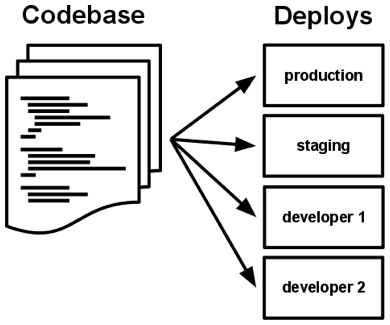
\includegraphics[width=\textwidth]{codebase-deploys.png}
							\caption{Codebasis mit unterschiedlichen Deploymentzweigen \cite{factor-codebase}}
						\end{figure}
					\end{columns}
				\end{frame}
			\subsection{II. Abhängigkeiten}
				\begin{frame}{II. Abhängigkeiten}
					Die meisten Programmiersprachen bieten ein System zur Verwaltung von Bibliotheken an.
					\begin{itemize}
						\item Site Package vs. Bundeling
						\item Abhängigkeitsdeklaration
						\item Isolation von Abhängigkeiten
						\item Systemwerkzeuge (z.B. bash, PowerShell, ...)
					\end{itemize}
				\end{frame}
			\subsection{III. Konfiguration}
				\begin{frame}{III. Konfiguration}
					Konfigurationen dürfen nicht im Quellcode definiert werden. Während die App selbst über viele Installationen hinweg statisch ist, unterscheiden sich die Konfigurationen je nach Deploy. Zugangsdaten und Netzwerkadressen sind Beispiele für derartige variable Daten die Ausgelagert werden müssen.
					\begin{itemize}
						\item Konfigurationsdateien (z.B. im yaml Format) - Nachteil: unbestimmter Ort
						\item Umgebungsvariablen - lassen eine klare Trennung von Code und Konfiguration zu und vermeiden Fehler. 
						\item Teilweise werden Umgebungsvariablen zur Strukturierung nach Deploy gruppiert. Nachteil: bei wachsenden Deploys Explosion der Anzahl von Umgebungsvariablen.
					\end{itemize} 
				\end{frame}
			\subsection{IV. Unterstützende Dienste}
				\begin{frame}{IV. Unterstützende Dienste}
					\begin{columns}
					\column{0.5\textwidth}
					Unterstützende Dienste sind alle nachgelagerten Dienste, welche über Netzwerk angesprochen werden. Beispiele für solche Dienste sind Datenbanken, Batchsysteme, Mailing, Cache, uvm.
					\begin{itemize}
						\item On-Premises vs. Cloud Dienste
						\item Unabhängig vom Deploy - Modular
					\end{itemize}
					\column{0.5\textwidth}
					\begin{figure}
						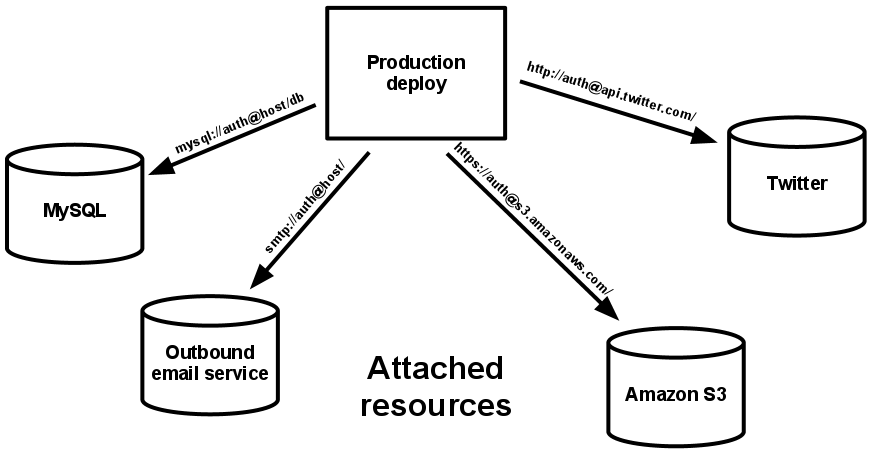
\includegraphics[width=\textwidth]{attached-resources.png}
						\caption{Hintergrunddienste einer Anwendung \cite{factor-subdienst}}
					\end{figure}
					\end{columns}
				\end{frame}
			\subsection{V. Build, Release, Run}
				\begin{frame}{V. Build, Release, Run}
					\begin{columns}
					\column{0.5\textwidth}
					Drei Schritte von der Codebase zum Deploy:
					\begin{enumerate}
						\item Build-Phase\newline $\rightarrow$ ausführbare Datei
						\item Release-Phase\newline $\rightarrow$ Konfiguration
						\item Run-Phase\newline $\rightarrow$ Ausführungsumgebung
					\end{enumerate}
					Strikte Trennung der Phasen!
					\column{0.5\textwidth}
					\begin{figure}
						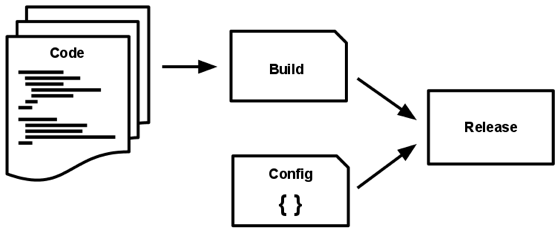
\includegraphics[width=\textwidth]{release.png}
						\caption{Hintergrunddienste einer Anwendung \cite{factor-release}}
					\end{figure}
					\end{columns}
				\end{frame}
			\subsection{VI. Prozesse}
				\begin{frame}{VI. Prozesse}
					Eine App benötigt im einfachsten Fall einen Prozess im Betriebssystem. Komplexere Anwendungen können jedoch sehr viele Prozesse benötigen.
					\begin{itemize}
						\item Daten werden in unterstützenden Diensten gespeichert
						\item RAM und Dateisystem können als Kurzzeit-Cache verwendet werden (eine Transaktion)
						\item Daten sind zwangsläufig unabhängig vom Prozess
					\end{itemize}
				\end{frame}
			%%%% Sidney %%%%
			\subsection{VII. Bindung an Ports}
				\begin{frame}{VII. Bindung an Ports}
					\begin{block}{Die Zwölf-Faktor-App läuft eigenständig}
						\begin{itemize}
							\item Unabhängig von einem gegebenfalls vorhandenem Webserver.
							\item Verarbeitung von HTTP innerhalb des Appcodes
							\item Bindet sich an einen Port und wartet dort auf Requests
							\item Auch andere Protokolle können angeboten werden
						\end{itemize}
					\end{block}
				\end{frame}
			\subsection{VIII. Nebenläufigkeit}
				\begin{frame}
					\frametitle{VIII. Nebenläufigkeit}
					\begin{columns}
						\column{0.5\textwidth}
							\begin{block}{Die Zwölf-Faktor-App wird anhand von Prozessen skaliert}
						\begin{itemize}
							\item Skalierung über die Anzahl der Prozesse
							\item Verwendung vom Prozessmanager des Systems zur Behandlung \newline von Triggern
						\end{itemize}
					\end{block}
					\column{0.5\textwidth}
					\begin{figure}[htpb]
						\centering
						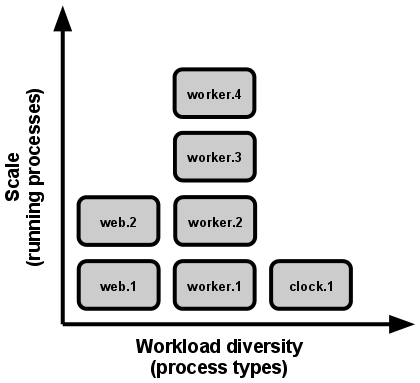
\includegraphics[width=\textwidth]{process-types.png}
						\caption{Skalierung mit Prozessen \cite{factor-concurrency}}
					\end{figure}
					\end{columns}
				\end{frame}
			\subsection{IX. Entsorgbarkeit}
			\begin{frame}
				\frametitle{IX. Entsorgbarkeit}
				\begin{block}{Die Prozesse der Zwölf-Faktor-App sind jederzeit entsorgbar}
					\begin{itemize}
						\item Die Prozesse können jederzeit gestartet und beendet werden
						\item Möglichst kleine Startzeiten
						\item Möglichst unproblematisches Beenden
						\item Robust gegenüber plötzlichen Tod
						\item Auf die Spitze getrieben: Crash-only design
					\end{itemize}
				\end{block}
			
			\end{frame}
			\subsection{X. Dev-Prod-Gleichheit}
				\begin{frame}
					\frametitle{X. Dev-Prod-Gleichheit}
					\begin{block}{Die Zwölf-Factor-App hat möglichst gleiche Entwicklungs- und Produktionsumgebungen}
						\begin{itemize}
							\item Zwölf-Factor-App ist für Continuous Deployment ausgelegt
							\item Gleiche Hintergrunddienste in beiden Umgebungen
						\end{itemize}
					\end{block}
					{\small
					\begin{tabular}{C{3cm}C{3cm}C{3cm}}
						& \textbf{Traditionelle App} & \textbf{Zwölf-Faktor-App} \\
						\textbf{Zeit \newline zwischen Deploys} & Tage -- Wochen & Stunden \\
						\textbf{Autoren und Verteiler} & unterschiedliche Personen & Dieselben Personen \\
						\textbf{Umgebungen} & Unterschiedlich & So gleich wie möglich
					\end{tabular}
					}
				
				\end{frame}
			\subsection{XI. Logs}
				\begin{frame}
					\frametitle{XI. Logs}
					\begin{block}{Die Zwölf-Factor -App sieht Logs als Eventströme}
					\begin{itemize}
						\item Die Zwölf-Faktor-App kümmert sich nicht um das Ziel der Ausgabedaten
						\item Es wird immer nach \texttt{stdout} geschrieben
						\item Die Ausführungsumgebung sammelt die Ausgaben aller Prozesse und kümmert sich um das Verarbeiten
						\item Möglichkeit, spezielle Loganalyse und -indizierungssysteme zu verwenden
					\end{itemize}	
					\end{block}
				\end{frame}
			\subsection{XII.\@ Administrationsprozesse}
			\begin{frame}
				\frametitle{XII. Administrationsprozesse}
				\begin{block}{Die Zwölf-Factor-App hat Administrationen als einmalige Vorgänge}
					\begin{itemize}
						\item Administrative Aufgaben laufen in derselben Umgebung wie die App
						\item Sie laufen in derselben Isolationsebene (Bundler bei Ruby, virtualenv bei Python etc.)
						\item Administrativer Code wird gemeinsam mit dem Anwendungscode ausgeliefert
					\end{itemize}
				\end{block}
				
			
			\end{frame}
		\section{Fazit}
			\subsection{Fazit und Kritik}
			\begin{frame}
				\frametitle{Fazit und Kritik}
				
				\begin{block}{Die 12 Factor App hat auch noch Schwächen\ldots}
					\begin{itemize}
					\item Gute Basis für die Entwicklung von Web Apps
					\item Kritik von Kevin Hoffman, Buch \enquote{Beyond the 12 Factor App}~\cite{beyond}
					\item Er erweitert die 12 Faktoren auf 15 und überarbeitet die vorhandenen
					\item Insbesondere Kritik am fehlenden Faktor Sicherheit, welches zentraler Bestandteil einer Web App sein muss
					\item Ansatz \enquote{API first} erlaubt eine bessere Integration
					\item Telemetrie erlaubt es, die App weiter auf das Nutzerverhalten zu optimieren
				\end{itemize}
				\end{block}
				
			
			\end{frame}
	\begin{frame}
		\frametitle{Quellen}
		\renewcommand{\bibfont}{\scriptsize}
		\printbibliography[heading=none]
	\end{frame}
\end{document}


